\documentclass[11pt,a4paper]{article}

% ── Page layout ───────────────────────────────────────
\usepackage[a4paper,margin=2.5cm]{geometry}
\usepackage{setspace}
\setstretch{1.15}

% ── Encoding & language ───────────────────────────────
\usepackage[utf8]{inputenc}
\usepackage[T1]{fontenc}
\usepackage[english]{babel}
\usepackage{microtype}

% ── Font: Helvetica ───────────────────────────────────
\usepackage[scaled=0.95]{helvet}
\renewcommand{\familydefault}{\sfdefault}

% ── Colour palette ────────────────────────────────────
\usepackage[table,xcdraw]{xcolor}
\definecolor{maincolor}{RGB}{100,155,0}
\definecolor{darkgray}{RGB}{60,60,60}
\definecolor{lightgray}{RGB}{245,245,245}

% ── Headers / footers ─────────────────────────────────
\usepackage{fancyhdr}
\pagestyle{fancy}
\fancyhf{}
\fancyhead[L]{\footnotesize\textcolor{darkgray}{Financial Tweet Sentiment Classification}}
\fancyhead[R]{\footnotesize\textcolor{darkgray}{NOVA IMS $\cdot$ Text Mining 2025/26}}
\fancyfoot[C]{\footnotesize\thepage}
\renewcommand{\headrulewidth}{0.4pt}
\renewcommand{\footrulewidth}{0pt}

% ── Section styling ───────────────────────────────────
\usepackage{titlesec}
\titleformat{\section}
  {\bfseries\color{maincolor}}{\thesection}{0.8em}{}
\titleformat{\subsection}
  {\color{maincolor}}{\thesubsection}{0.8em}{}
\titleformat{\subsubsection}
  {\bfseries\color{darkgray}}{\thesubsubsection}{0.8em}{}

\titlespacing*{\section}{0pt}{8pt}{4pt}
\titlespacing*{\subsection}{0pt}{6pt}{3pt}
\titlespacing*{\subsubsection}{0pt}{4pt}{2pt}

% ── Math ───────────────────────────────────────────────
\usepackage{amsmath, amssymb}

% ── Graphics / floats ─────────────────────────────────
\usepackage{graphicx}
\usepackage{float}
\usepackage{placeins}
\graphicspath{{results/figures/}}

% ── Tables ────────────────────────────────────────────
\usepackage{booktabs}
\usepackage{multirow}
\usepackage{array}
\usepackage{tabularx}
\usepackage{colortbl}

\newcommand{\tH}[1]{\textcolor{maincolor}{\textbf{#1}}}
\newcommand{\gmid}{\arrayrulecolor{maincolor}\midrule\arrayrulecolor{black}}

% ── Captions ──────────────────────────────────────────
\usepackage{caption}
\captionsetup{
  font=small,
  labelfont={bf,color=maincolor},
  skip=4pt
}

% ── Lists ─────────────────────────────────────────────
\usepackage{enumitem}
\setlist[itemize]{
  noitemsep,
  topsep=2pt,
  parsep=0pt,
  partopsep=0pt,
  leftmargin=1.4em,
  label=\textcolor{maincolor}{\textbullet}
}

% ── Paragraph spacing ─────────────────────────────────
\setlength{\parindent}{0pt}
\setlength{\parskip}{3pt}

% ── Hyperlinks ────────────────────────────────────────
\usepackage[
  colorlinks=true,
  linkcolor=maincolor,
  citecolor=darkgray,
  urlcolor=maincolor,
  pdfborder={0 0 0}
]{hyperref}

% ── Convenience ───────────────────────────────────────
\newcommand{\ttt}[1]{\texttt{\hyphenchar\font=`\-\relax #1}}

% ── Distilled single-model metrics (extra work) — single source of truth ──
\newcommand{\distf}{0.9139}    % OOF macro-F1 of the distilled student (12 epochs)
\newcommand{\distacc}{0.9334}  % OOF accuracy of the distilled student

\begin{document}

% ── Typesetting tolerance: absorb long monospace tokens, avoid margin overflow ──
\tolerance=2000
\emergencystretch=3em
\hfuzz=1pt

% ── Title block ──────────────────────────────────────────────────
\thispagestyle{fancy}
\begin{center}
  {\LARGE\bfseries\color{maincolor} Financial Tweet Sentiment Classification}\\[3pt]
  {\large\color{darkgray} Multiclass Sentiment Analysis of Financial Social Media Text}\\[8pt]
  {\normalsize Text Mining --- MSc in Data Science and Advanced Analytics}\\[1pt]
  {\normalsize NOVA Information Management School (NOVA IMS)}\\[5pt]
  {\normalsize \textbf{Group 33} \quad$\cdot$\quad Academic Year 2025/2026 \quad$\cdot$\quad June 2026}
\end{center}
\vspace{2pt}
{\color{maincolor}\rule{\linewidth}{0.6pt}}
\vspace{4pt}

% ── Abstract ─────────────────────────────────────────────────────
\section*{Abstract}
This report presents a multiclass sentiment classification system for financial tweets,
distinguishing three market stances: Bearish (0), Bullish (1), and Neutral (2). The dataset
comprises 9{,}543 labelled training tweets with pronounced class imbalance (Neutral 64.7\%,
Bullish 20.1\%, Bearish 15.1\%; imbalance ratio 4.28:1) and substantial text corruption: 7.0\% of
tweets carry UTF-8 mojibake and 16.4\% end in truncation artefacts. We systematically evaluate
seven text preprocessing techniques, eleven feature representations --- spanning sparse TF--IDF,
Word2Vec, GloVe--Twitter, FinBERT, SBERT and Twitter--RoBERTa embeddings --- and twelve model
families under a common stratified cross-validation protocol (10-fold for all transformer
fine-tuning, seed 42). Frozen-embedding classifiers tuned with Optuna plateau around macro-F1 0.80.
A \textbf{transformer backbone search} over nine fine-tuned encoders shows that domain-matched
pre-training dominates model size: a 110M-parameter \textbf{FinBERT} variant pre-adapted to
financial Twitter text reaches an out-of-fold macro-F1 of \textbf{0.9082}, beating DeBERTa-v3-large
(435M, 0.8889). As extra work, a weighted soft-vote \textbf{ensemble} of eight encoders --- with
weights found by exhaustive out-of-fold grid search --- attains \textbf{0.9201}, a statistically
significant gain over the best individual model (bootstrap 95\% CI of the difference:
$[+0.007, +0.017]$). The instructor confirmed that an ensemble is an acceptable final solution
when it forms a single integrated end-to-end pipeline, so this weighted soft-vote ensemble is our
\textbf{submitted solution}. We additionally \textbf{distil} it into one FinBERT student (Hinton
et al., 2015) at OOF macro-F1 \textbf{\distf} (extra work), showing the ensemble compresses into a
single 110M-parameter model. We additionally show that a fine-tuned \textbf{GPT-2
decoder} classifies at macro-F1 0.7724 (whereas few-shot prompting collapses to the majority
class), and that an offline \textbf{agentic workflow} adaptively routes tweets between VADER,
LightGBM/SBERT and FinBERT with conversational explanations.

\vspace{2pt}
{\footnotesize\tH{Keywords:}~ Financial sentiment analysis, tweet classification, FinBERT
fine-tuning, model selection, ensemble distillation, decoder classification, LangChain agent.}

% ── 1. Introduction ──────────────────────────────────────────────
\section{Introduction}
Social media platforms --- particularly Twitter/X --- have become a primary channel through which
retail and institutional investors express and discover market sentiment. Automated classification
of financial tweets into Bearish, Bullish and Neutral stances enables real-time signal generation
for algorithmic trading, risk monitoring and investor-sentiment tracking (Bollen et al., 2011;
Antweiler \& Frank, 2004).

This work addresses multiclass financial sentiment classification --- a text-categorization
problem in the classical sense of Sebastiani (2002) --- under significant class imbalance
(ratio 4.28:1). We explore the full NLP pipeline --- from raw text through feature engineering to
model selection and hyperparameter tuning --- following the Text Mining curriculum at NOVA IMS. All
models are trained \emph{only} on the provided training corpus. The remainder of the report is
organised as follows: Section~2 explores the dataset; Section~3 analyses preprocessing; Section~4
describes feature engineering; Section~5 presents the classification models, including the backbone
search and the fine-tuned encoder/decoder; Section~6 reports results and error analysis; Section~7
details the agentic workflow (Extra Challenge~2); Section~8 concludes.

\textbf{Course alignment.} Every stage follows the Text Mining curriculum: the NLP pipeline and
text preprocessing (Lecture~1, Lab~1); n-grams, TF--IDF and distance metrics (Lecture~2-Extra);
word2vec word embeddings and their semantic geometry (Lecture~2, Lab~2); attention and Transformer
\emph{encoders} (Lecture~4, Lab~4); and \emph{decoder} LLMs, encoder-based classification and
\emph{Agentic AI} (Lecture~6, Lab~5; Alammar \& Grootendorst, 2024).

% ── 2. Data Exploration ──────────────────────────────────────────
\section{Data Exploration}
The dataset consists of 9{,}543 labelled training tweets and 2{,}388 unlabelled test tweets from
financial Twitter discourse. Each tweet references one or more publicly-listed securities and
expresses a market stance.

\subsection{Class Distribution}
Figure~\ref{fig:classdist} illustrates the severe class imbalance. Neutral tweets dominate (64.7\%),
consistent with most financial discourse being non-directional. Bearish tweets (15.1\%) are less
frequent than Bullish (20.1\%), reflecting a structural optimism bias in financial social media
(Antweiler \& Frank, 2004). To address imbalance, all models use \texttt{class\_weight='balanced'}
(or an inverse-frequency-weighted loss) and evaluation relies on \textbf{macro-F1} as the primary
metric, which weights all three classes equally regardless of support.

\begin{figure}[H]
  \centering
  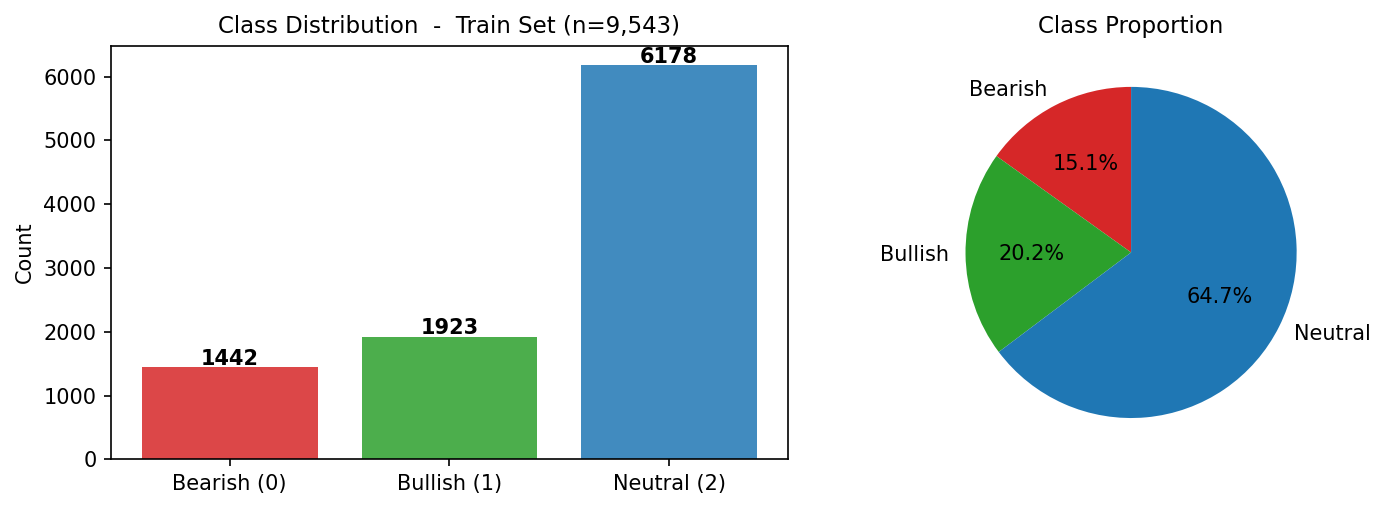
\includegraphics[width=0.95\linewidth]{report_class_dist.png}
  \caption{Class distribution of the training set: absolute counts (left) and proportions (right).}
  \label{fig:classdist}
\end{figure}

\subsection{Linguistic Characteristics}
Tweets have a mean length of 12.2 words (maximum 32), consistent with Twitter's character limit. Key
Twitter-specific features include cashtags (\$AAPL, \$TSLA), hashtags (\#earnings, \#bearish),
mentions (@analyst) and URLs. Bullish tweets contain more cashtags on average (0.34 vs.\ 0.22 for
Bearish), suggesting that positive sentiment correlates with specific stock discussion. The most
discriminative terms per class are: \textbf{Bearish} --- `down', `miss', `cut', `bearish';
\textbf{Bullish} --- `beats', `strong', `upgraded', `buy'; \textbf{Neutral} --- `flat',
`unchanged', `stable'. Per-class word clouds are included in the accompanying notebook.

\subsection{Text-Quality Audit: Mojibake and Truncation}
A character-level audit reveals that the corpus is \emph{corrupted at source}: 7.0\% of training
tweets contain UTF-8 mojibake (byte sequences decoded with the wrong codec, e.g.\
\texttt{\detokenize{’}} instead of an apostrophe), 16.4\% end in truncation artefacts
(\texttt{...}/replacement characters cutting the sentence mid-token), and 46.8\% carry URLs with no
sentiment value. In total, 50.1\% of tweets are altered by our repair step. Corruption is not
uniform across classes (Neutral 8.7\%, Bearish 5.5\%, Bullish 2.9\%), so leaving it unfixed injects
class-correlated noise. This finding motivates the \texttt{fix\_text} preprocessing technique
(Section~3.1) based on the \texttt{ftfy} library (Speer, 2019). A complementary duplicate audit
finds \emph{zero} exact duplicates in the training set; after normalisation, 2.1\% of tweets are
near-duplicates (URL/encoding variants of the same post), of which three groups carry
\emph{conflicting labels} --- direct evidence of annotation noise --- and 42 test tweets have a
near-identical training counterpart (a property of the provided split). No rows are dropped.
Finally, a cashtag ablation (15.0\% of tweets contain \$AAPL-style tags) shows that ticker
\emph{identity} carries no sentiment signal: keeping cashtags, collapsing them to a generic token,
or removing them entirely all score within one standard deviation (0.7149--0.7161, leak-free
protocol). Mapping tickers to company names was therefore rejected --- it would re-introduce
identity as rare tokens with no expected gain and, for the transformer, shift inputs away from the
pre-training distribution of FinBERT-fintwitter, which contains native cashtags. Finally, \emph{adversarial validation} --- a classifier trained to distinguish training
from test tweets --- yields AUC 0.486 ($\approx$0.5), and all surface statistics match across the
two sets: the test set is statistically indistinguishable from training, so our out-of-fold
estimates are a reliable proxy for test performance.

\subsection{Lexicon Limits: VADER by Class}
Scoring every tweet with VADER (Hutto \& Gilbert, 2014) exposes why general-purpose lexicons fail
on financial text: among \emph{Neutral} tweets, 32.2\% have a positive VADER compound and 18.4\% a
negative one --- over half of the majority class looks polarised to a lexicon. Financial wording
(``raised'', ``beats'', ``cut'', ``misses'') is factual news vocabulary, not opinion. This
quantifies the need for domain-specific models (FinBERT) over lexicon or generic baselines, and is
revisited by the agentic workflow in Section~7, which only trusts VADER when its signal is strong.

\subsection{EDA-to-Modelling Decisions}
The exploratory analysis is not only descriptive; it directly determines the modelling choices.
\begin{table}[H]
  \centering
  \scriptsize
  \setlength{\tabcolsep}{5pt}
  \begin{tabularx}{\linewidth}{@{}>{\raggedright\arraybackslash}p{0.27\linewidth}
                                >{\raggedright\arraybackslash}p{0.33\linewidth}
                                >{\raggedright\arraybackslash}X@{}}
    \toprule
    \tH{Finding} & \tH{Evidence} & \tH{Modelling consequence} \\
    \gmid
    Severe class imbalance & Neutral 64.7\%, Bullish 20.1\%, Bearish 15.1\% &
    Stratified folds, class-weighted losses and macro-F1 as the primary metric. \\
    Short, information-dense tweets & Mean 12.2 words, maximum 32 words &
    Transformer max length 128 covers the corpus (max 33 words) with subword headroom. \\
    Financial tokens carry sentiment & Cashtags, analyst actions, earnings and target-price terms &
    Raw text is preserved for the final transformer; aggressive cleaning is tested but not assumed. \\
    URL/mention boilerplate is common & URLs appear in 46.8\% of the tweets &
    Regex cleaning is evaluated for sparse baselines, while tweet-specialised tokenizers handle raw text. \\
    Corpus is corrupted at source & 7.0\% mojibake, 16.4\% truncation artefacts, class-correlated &
    New \texttt{fix\_text} repair step (ftfy + artefact/URL cleanup), ablated for sparse models and transformers. \\
    Lexicons mis-read financial news & 50.6\% of Neutral tweets look polarised to VADER &
    Domain-matched encoders (FinBERT) prioritised in the backbone search; VADER demoted to agent baseline. \\
    \bottomrule
  \end{tabularx}
  \caption{How EDA findings are translated into concrete modelling choices.}
  \label{tab:eda_decisions}
\end{table}

\subsection{Corpus Split and Validation Protocol}
To satisfy the corpus-split requirement without wasting labelled data, every experiment uses
\textbf{stratified $k$-fold cross-validation} on the 9{,}543 labelled tweets
(\texttt{StratifiedKFold}, \texttt{shuffle=True}, \texttt{random\_state=42}). Stratification keeps
the Bearish/Bullish/Neutral proportions stable in each validation fold, which is essential under the
4.28:1 imbalance. All transformer fine-tuning and the final solution use \textbf{10 folds} (train
on 90\%, validate on 10\%), which both enlarges each training split and stabilises the averaged
test prediction; the broad classical-ML comparison (68 model$\times$feature combinations,
Section~5.1) uses 5 folds for tractability. Out-of-fold (OOF) predictions give honest, leak-free
macro-F1 on the full corpus, and the fold-level test probability vectors are averaged to produce
\texttt{pred\_33.csv}. The identical seed and splitter make every OOF score in this report directly
comparable within its protocol.

% ── 3. Data Preprocessing ────────────────────────────────────────
\section{Data Preprocessing}
We implement six preprocessing techniques following the NLTK-based approach from course Lab~1 and
the tweet-tokenisation practice from the extra TF--IDF lab. Crucially, preprocessing is treated as an
\emph{empirical question}: every variant is measured under the same 5-fold protocol before deciding
what enters the final pipeline.

\subsection{Preprocessing Pipeline}
\begin{itemize}
  \item \tH{T1 --- Twitter noise cleaning.} Regex removal of URLs and mentions
  ($\to$ \texttt{USER}); hashtag-symbol stripping; cashtags mapped to \texttt{TICKER\_X}.
  \item \tH{T2 --- Unicode normalisation.} NFKD decomposition then ASCII encoding.
  \item \tH{T3 --- Stop-word removal.} NLTK English list, negations preserved
  (\{not, no, never, neither, nor, none\}) --- critical for sentiment (Manning et al., 2008).
  \item \tH{T4 --- WordNet lemmatisation.} POS-aware: `beaten' $\to$ `beat', `falling' $\to$ `fall'.
  \item \tH{T5 --- Snowball stemming.} More aggressive: `earnings' $\to$ `earn'.
  \item \tH{T6 --- TweetTokenizer.} \texttt{reduce\_len=True}, \texttt{strip\_handles=True}.
  \item \tH{T7 --- fix\_text (encoding repair).} Motivated by the text-quality audit
  (Section~2.3): \texttt{ftfy} mojibake repair (Speer, 2019), removal of end-of-tweet truncation
  artefacts and of sentiment-free URLs. Unlike T1--T6, this step \emph{restores} signal rather than
  removing it, and alters 50.1\% of tweets.
\end{itemize}

Example transformations are shown in the notebook: URLs and mentions become generic tokens, cashtags
retain the ticker identity, negations survive stop-word removal, and lemmatisation/stemming reduce
inflected forms. This demonstrates compliance with the preprocessing requirement while also exposing
the main trade-off: cleaning removes noise, but may also remove finance-specific signal.

\subsection{Ablation Study}
Each configuration is evaluated with Logistic Regression ($C=1.0$) and TF--IDF (10{,}000 vocabulary)
under 5-fold stratified CV.

\begin{figure}[H]
  \centering
  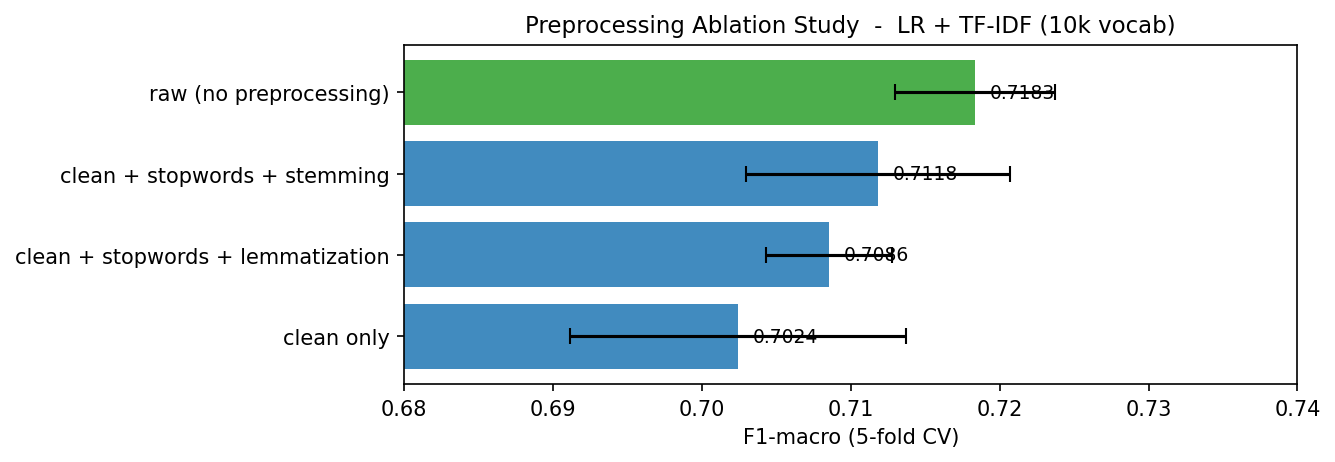
\includegraphics[width=0.86\linewidth]{report_ablation.png}
  \caption{Preprocessing ablation: macro-F1 by configuration (green = best). Encoding repair
  (fix\_text) edges out raw text; every destructive pipeline hurts.}
  \label{fig:ablation}
\end{figure}

\begin{table}[H]
  \centering
  \small
  \setlength{\tabcolsep}{8pt}
  \begin{tabularx}{0.86\linewidth}{@{}>{\raggedright\arraybackslash}X r r@{}}
    \toprule
    \tH{Preprocessing configuration} & \tH{Macro-F1} & \tH{Std} \\
    \gmid
    \rowcolor{lightgray} light cleaning only (URL/ticker tokens, lowercase) & \textbf{0.7179} & 0.0038 \\
    raw (no preprocessing)                                   & 0.7152 & 0.0040 \\
    raw + fix\_text (ftfy repair)                            & 0.7149 & 0.0032 \\
    clean + stop-words + lemmatisation                       & 0.7068 & 0.0045 \\
    clean + stop-words + stemming                            & 0.7062 & 0.0080 \\
    \bottomrule
  \end{tabularx}
  \caption{Preprocessing ablation (5-fold CV, LR + TF--IDF, vectoriser fitted \emph{inside} each
  fold). The top three variants are tied within one standard deviation; stemming and lemmatisation
  cost $\sim$1pp.}
  \label{tab:ablation}
\end{table}

\textbf{Key finding:} for sparse models, light or no preprocessing variants are statistically
\emph{tied} (0.715--0.718), while aggressive stemming/lemmatisation \emph{destroys} signal
($-$1pp) --- ticker symbols (\$AAPL), analyst-firm names and domain vocabulary (`downgrade',
`EPS beat', `guidance raise') are discriminative features (Go et al., 2009). The value of
fix\_text does not show at TF--IDF level (the vectoriser tokenises encoding artefacts away) but
emerges with fine-tuned transformers, whose subword vocabularies are sensitive to corrupted bytes:
\textbf{+0.26pp} on FinBERT (0.9056 $\to$ 0.9082) and +0.07pp on DeBERTa-v3-large (0.8882 $\to$
0.8889) under the 10-fold protocol (full ablation in \nolinkurl{tm_tests_33.ipynb}, Section~5g).
The final pipeline therefore feeds the transformer \emph{repaired raw text}: fix\_text only, no
destructive cleaning. (Methodological note: this table was re-measured with the vectoriser fitted
inside each fold after an internal leakage audit; the conventional fit-once protocol used in the
broad 68-combination comparison of Section~5.1 inflates sparse baselines uniformly by
$\approx$0.4pp without changing any ranking.)

% ── 4. Feature Engineering ───────────────────────────────────────
\section{Feature Engineering}

Feature engineering converts each tweet into a numerical vector that a classifier can process.
Eleven representations were built across four families, progressing from sparse and interpretable
baselines to rich contextual embeddings.

\begin{table}[h]
\centering
\small
\begin{tabular}{llrll}
\toprule
\textbf{Family} & \textbf{Representation} & \textbf{Dim} & \textbf{Alignment} & \textbf{Rubric} \\
\midrule
Sparse  & BoW (binary)                  & $\leq$20k & —                        & Base \\
        & TF-IDF unigrams               & $\leq$20k & —                        & Base \\
        & TF-IDF unigrams+bigrams       & $\leq$50k & Financial expressions    & Base \\
        & TF-IDF char 3–5grams          & $\leq$30k & Twitter spelling noise   & Base \\
\midrule
Static  & Word2Vec Skip-gram            & 200       & In-domain corpus         & Base \\
        & Word2Vec CBOW                 & 200       & In-domain corpus         & Base \\
        & GloVe-Twitter-100             & 100       & Twitter (2B tweets)      & Base \\
\midrule
Contextual & FinBERT CLS               & 768       & Finance                  & Base (obligatory) \\
           & SBERT all-mpnet           & 768       & General-purpose          & \textbf{EXTRA} \\
           & Twitter-RoBERTa CLS       & 768       & Twitter (58M tweets)     & \textbf{EXTRA} \\
\midrule
Hand-crafted & Financial features      & 14        & Finance + Twitter surface & Base \\
\bottomrule
\end{tabular}
\caption{Feature representations implemented. Representations marked \textbf{EXTRA} are
additional Transformer Encoder methods beyond the base requirement.}
\label{tab:features}
\end{table}

\subsection{Sparse Representations (BoW and TF-IDF)}

Both BoW and TF-IDF represent each tweet as a vector with one position per vocabulary word.
Binary BoW records word presence/absence and serves as an interpretable lower bound.
TF-IDF improves on this by weighting each word by how distinctive it is across the corpus:
rare financial terms like \textit{downgrade} or \textit{beats} receive high weight while common
words are suppressed. The unigram+bigram variant adds two-word sequences to capture financial
expressions such as \textit{price target} or \textit{earnings beat} that vanish at the word
level. The character 3–5gram variant operates on overlapping character sequences, making the
representation robust to Twitter spelling noise (\textit{bullllish} and \textit{bullish} share
most character sequences and produce similar vectors). All sparse methods share a fundamental
limitation: they treat words independently, with no notion of order or context.

\subsection{Static Word Embeddings (Word2Vec and GloVe)}

Word2Vec learns a dense vector per word by training a neural network to predict words from
their context, so semantically related words end up numerically close : \textit{bullish} and
\textit{optimistic} become neighbours in the vector space. Skip-gram predicts context from the
centre word and handles rare financial terms better; CBOW predicts the centre word from context
and is stronger on frequent vocabulary. Both 200-dimensional models are trained on the 9,543
in-domain tweets. GloVe-Twitter-100, pre-trained on 2 billion tweets,
provides broader coverage of informal Twitter language at the cost of financial specificity.
Each tweet is represented by mean pooling its token vectors. The key remaining limitation is
context-insensitivity: the vector for \textit{cut} is identical in \textit{Fed cuts rates} and
\textit{analyst cuts target}, despite opposite implications.

\subsection{Contextual Transformer CLS Embeddings}

Transformer encoders solve context-insensitivity by reading the entire sequence through
self-attention, where each word's representation is shaped by all other words in the tweet.
A special \texttt{[CLS]} token accumulates this information across all encoder layers, producing
a 768-dimensional contextualised summary of the tweet. Three encoders
are used in frozen mode (weights not updated) as pure feature extractors.

\textbf{FinBERT} (Araci, 2019), fine-tuned on financial news and earnings reports, provides
direct domain alignment for financial vocabulary and sentiment. However, its training corpus
is formal text, which limits its ability to handle the informal language, abbreviations, and
noise typical of Twitter.

\textbf{SBERT all-mpnet-base-v2} (Reimers \& Gurevych, 2019) is trained with contrastive
objectives, producing embeddings well-suited for similarity-based classifiers — however, it
has no alignment with either financial text or Twitter language.
\textbf{This constitutes Extra Work \#1 under the Feature Engineering criterion.}

\textbf{Twitter-RoBERTa} (Barbieri et al., 2020), pre-trained on 58M tweets, handles informal
language, abbreviations, and the noisy writing style typical of Twitter — however, its
pre-training corpus is general Twitter data, not financial text specifically, so it may miss
domain-specific vocabulary.
\textbf{This constitutes Extra Work \#2 under the Feature Engineering criterion.}

PCA projections of the three encoder spaces confirmed that FinBERT (47.1\% variance explained)
and Twitter-RoBERTa (52.0\%) produce visibly cleaner class separation than SBERT (7.7\%).
This diagnostic is not used as a model-selection criterion: PCA measures how much variance a
two-dimensional projection preserves, not supervised class-discriminative power. Model choice in
Section~5 is therefore based on validation macro-F1.

\subsection{Financial Hand-crafted Features}

A 14-dimensional vector captures Twitter surface signals that no unsupervised embedding learns
by design: VADER sentiment scores (\textit{pos}, \textit{neg}, \textit{neu}, \textit{compound};
Hutto \& Gilbert, 2014), cashtag, hashtag, mention and URL counts, word and character count,
exclamation and question marks, all-caps ratio, and Flesch readability score. A fusion
experiment concatenating these features with SBERT embeddings (782 dimensions total) yielded
a marginal gain of +0.0032 F1-macro, suggesting SBERT already captures most surface signal
implicitly: a useful negative result that informed the final feature-set decision. SBERT is used
here as a conservative semantic baseline for the hand-crafted-feature ablation; the stronger
RoBERTa and FinBERT encoders are evaluated separately in the classical and fine-tuned model
comparisons, where the final selection is made by supervised validation performance.

\textbf{Reproducibility.} All eleven representations are produced by a single deterministic script,
\nolinkurl{scripts/generate_features.py} (seed 42), which executes the functions in
\nolinkurl{src/features.py} and writes the dense matrices to \nolinkurl{data/processed/} and the
fitted vectorisers to \nolinkurl{results/models/}. Because the dense embeddings total 153\,MB they
are not bundled with the submission; the feature-loading cell in \nolinkurl{tm_tests_33.ipynb}
regenerates them on demand.

% ── 5. Classification Models ─────────────────────────────────────
\section{Classification Models}
All models are evaluated via stratified cross-validation (\texttt{StratifiedKFold},
\texttt{random\_state=42}) with macro-F1 as the primary metric --- 5 folds for the broad classical
sweep (Section~5.1), 10 folds for all transformer fine-tuning and the final solution
(Sections~5.2--5.4). Within each protocol the identical split makes the out-of-fold (OOF) scores
directly comparable.

\subsection{Traditional ML Models}
\begin{itemize}
  \item \tH{Na\"ive Bayes.} MultinomialNB ($\alpha=1.0$) and ComplementNB ($\alpha=0.5$) on
  BoW / TF--IDF; ComplementNB targets imbalance (Rennie et al., 2003).
  \item \tH{Logistic Regression.} $L_2$ (SAGA), $C \in \{0.1, 1.0, 10.0\}$, all feature sets.
  \item \tH{Linear SVM.} CalibratedClassifierCV(LinearSVC), $C \in \{0.1, 1.0\}$.
  \item \tH{KNN.} $k \in \{5, 15\}$, cosine distance, dense embeddings.
  \item \tH{MLP.} $(256,128)$ and $(512,256,128)$, ReLU, early stopping.
  \item \tH{Random Forest / XGBoost / LightGBM.} 100 and 300 estimators; LightGBM is the strongest
  traditional learner on dense embeddings.
\end{itemize}

\subsection{Transformer Encoder Fine-tuning + Backbone Search}
Whereas Section~4.3 used the encoders only as \emph{frozen} embeddings, here the full encoder is
fine-tuned end-to-end (Devlin et al., 2019) --- the single largest lever in this study. Using the
Hugging Face Hub for \textbf{model selection}, we shortlist nine candidate configurations and
fine-tune each under the identical 10-fold protocol: 5--10 epochs, learning rate
$5\times10^{-6}$--$10^{-5}$ with cosine warmup, batch 8--16 (gradient accumulation to effective 32
for the large models), max length 128, AdamW, gradient clipping 1.0, inverse-frequency
class-weighted cross-entropy with label smoothing 0.05, fp16 mixed precision with loss scaling, and
best-checkpoint-per-fold selection on validation F1 (NVIDIA RTX~5070).
Table~\ref{tab:backbones} reports the comparison.

\begin{table}[H]
  \centering
  \footnotesize
  \setlength{\tabcolsep}{5pt}
  \begin{tabularx}{\linewidth}{@{}>{\raggedright\arraybackslash}X r r r@{}}
    \toprule
    \tH{Backbone (fine-tuned end-to-end, 10-fold)} & \tH{Params} & \tH{OOF F1} & \tH{Acc.} \\
    \gmid
    \rowcolor{lightgray} \textbf{FinBERT-fintwitter, 10 ep + fix\_text} & 110M & \textbf{0.9082} & \textbf{0.9293} \\
    FinBERT-fintwitter, 7 ep + LLRD 0.9 + fix\_text         & 110M & 0.9080 & 0.9285 \\
    FinBERT-fintwitter, 10 ep (raw text)                    & 110M & 0.9056 & 0.9275 \\
    FinBERT-fintwitter, 7 ep                                & 110M & 0.9049 & 0.9264 \\
    FinBERT-fintwitter, 5 ep                                & 110M & 0.9025 & 0.9243 \\
    twitter-roberta-large-topic-sentiment (prev.\ submission) & 355M & 0.8943 & 0.9141 \\
    DeBERTa-v3-large, 6 ep + fix\_text (He et al., 2021)$^\dagger$ & 435M & 0.8889 & 0.9107 \\
    DeBERTa-v3-large, 6 ep                                  & 435M & 0.8882 & 0.9100 \\
    DeBERTa-v3-base finance, 8 ep + fix\_text               & 184M & 0.8715 & 0.8947 \\
    \bottomrule
  \end{tabularx}
  \caption{Transformer backbone search (identical 10-fold protocol, seed 42). The shaded
  FinBERT-fintwitter is the best individual encoder and the distillation student of Section~5.3.
  LLRD = layer-wise learning-rate decay. $^\dagger$DeBERTa-v3 requires fp32 master weights with
  loss scaling --- its disentangled attention overflows in plain fp16.}
  \label{tab:backbones}
\end{table}

The decisive factor is \textbf{domain-matched pre-training, not size}: the winning encoder
(\ttt{nickmuchi/finbert-tone-finetuned-fintwitter-classification}) is a 110M-parameter FinBERT
(Araci, 2019) already adapted to financial-Twitter text, and it outperforms a four-times-larger
DeBERTa-v3-large by $\sim$2pp. We replace its classification head with a fresh 3-class head and
fine-tune the complete network. Best individual configuration: OOF macro-F1 \textbf{0.9082}
($\pm$0.0098), accuracy 0.9293, precision 0.9008, recall 0.9163 --- a \textbf{+0.1061} gain over
the 0.8021 frozen-embedding baseline and +0.0139 over our previous submission candidate
(Twitter--RoBERTa-large, 0.8943). Two further observations: (i) the fix\_text repair contributes
+0.26pp at no architectural cost (Section~3.2); (ii) LLRD ties the best model (0.9080) but trains
with different layer dynamics --- useful diversity for the ensemble below.

\subsection{Weighted Soft-Vote Ensemble (Submitted) and Distillation (Extra Work)}
\label{sec:distill}
The backbone search leaves us with several strong, partially decorrelated encoders. We combine them
by \textbf{weighted soft-voting}: test probabilities are averaged with per-model
weights found by \emph{exhaustive} OOF grid search --- all $2^8$ model subsets crossed with weights
$\{0.25, 0.5, 0.75, 1.0\}$, evaluated on leak-free OOF predictions. The optimum keeps eight models
(four at weight 1.0, three at 0.75, one at 0.5) and reaches OOF macro-F1 \textbf{0.9201} ---
+1.19pp over the best individual encoder. A paired bootstrap over the 9{,}543 OOF predictions
(1{,}000 resamples) puts the 95\% confidence interval of this gain at $[+0.0066, +0.0172]$,
excluding zero: the improvement is real, not resampling noise (Section~6.3).

The instructor confirmed (e-mail, June 2026) that an ensemble is an acceptable final solution
provided it is \emph{a single integrated end-to-end pipeline that consumes the input in a unified
way through to the prediction}; \nolinkurl{tm_final_33.ipynb} is exactly such a weighted soft-vote
pipeline, so \textbf{this ensemble is the submitted solution} (\nolinkurl{pred_33.csv}). As
further extra work we also \textbf{distil} the ensemble (Hinton et al., 2015): the eight-model
ensemble becomes the
\emph{teacher}, and a single FinBERT-fintwitter student is trained on the combined objective
\[
\mathcal{L} \;=\; (1-\alpha)\,\mathrm{CE}_{\text{weighted}}(y, p_s)
\;+\; \alpha\, T^2\, \mathrm{KL}\!\left(p_t^{(T)} \,\|\, p_s^{(T)}\right),
\qquad \alpha = 0.5,\; T = 2,
\]
where the teacher targets $p_t$ are the ensemble's \emph{out-of-fold} probabilities --- each
training sample's soft target comes from folds that never saw that sample, so the distillation
itself is leakage-free. Training otherwise mirrors the 10-fold recipe of Section~5.2, extended to
12 epochs: because soft targets regularise, the student benefits from longer training (+0.18pp on
a 3-fold proxy, confirmed on the full protocol). A grid search
over the distillation hyperparameters ($\alpha \in \{0.5, 0.7, 0.9, 1.0\}$, $T \in \{2, 3\}$,
3-fold proxy) confirmed $\alpha{=}0.5$, $T{=}2$ as optimal; R-Drop consistency regularisation and
post-hoc per-class probability scaling were also evaluated and \emph{rejected}, as their held-out
gains were within noise --- consistent
with the calibration analysis of Section~6.3. The distilled
student reaches OOF macro-F1 \textbf{\distf} (accuracy \distacc) --- recovering 48\% of the
ensemble's gain in a single 110M-parameter model, itself a statistically significant improvement
over the best conventionally-trained encoder (paired bootstrap 95\% CI: $[+0.0023, +0.0094]$).
It is reported as \textbf{extra work} --- a demonstration that the submitted ensemble can be
compressed into a single model with minimal loss of accuracy.

\subsection{Decoder Model --- Fine-tuned GPT-2 (Extra Work)}
As decoder-based extra work we use a \emph{decoder} (causal) language model for classification.
\textbf{GPT-2} (Radford et al., 2019) is fine-tuned end-to-end with a sequence-classification head
(\texttt{GPT2ForSequenceClassification}, which pools the last non-pad token) under the same 5-fold
protocol. It reaches an OOF macro-F1 of \textbf{0.7724} (accuracy 0.8125) --- a genuine
decoder-for-classification result. For completeness we also tried \emph{few-shot prompting} of GPT-2
in the in-context-learning style of GPT-3 (Brown et al., 2020), using verbalizer likelihood scoring
with contextual calibration (Zhao et al., 2021); it collapses to the majority class (macro-F1
$\approx$ 0.25), empirically showing that a 124M decoder is too weak to classify zero/few-shot and
that fine-tuning is the correct route.

\subsection{Hyperparameter Tuning --- Optuna}
Optuna (Akiba et al., 2019) with a TPE sampler and median pruner runs 50 trials over LightGBM
hyperparameters; the best frozen-embedding configuration reaches macro-F1 0.8021 (RoBERTa features).
A second study tunes Logistic-Regression $C$ on TF--IDF bigrams; a soft-voting LR+SVC ensemble
provides a strong sparse baseline.

\subsection{Stacking Ensemble (Extra Work)}
As additional work we build a stacked generalisation (Wolpert, 1992): six base learners
(Optuna-tuned LightGBM on RoBERTa, MLP on SBERT, XGBoost on RoBERTa, LightGBM on FinBERT, LR on
TF--IDF bigrams, and a fine-tuned Twitter--RoBERTa) emit out-of-fold probabilities concatenated into
an 18-dimensional meta-feature matrix on which a Logistic-Regression meta-learner is trained. Because
every base learner shares the identical fold split, the meta-features are leakage-free. The stack
reaches OOF macro-F1 \textbf{0.8483} --- strong at the time, but ultimately surpassed both by the
individually fine-tuned encoders of Section~5.2 and by the soft-vote ensemble of Section~5.3, which
combines stronger, more diverse base models.

% ── 6. Results ───────────────────────────────────────────────────
\section{Results and Evaluation}

\subsection{Model Comparison}
Figure~\ref{fig:results} ranks the top configurations and Table~\ref{tab:results} lists the top
models. The eight-encoder ensemble (extra work) tops the ranking at OOF macro-F1 \textbf{0.9201};
and is our \textbf{submitted solution}; the distilled single model (extra work) follows at
\textbf{\distf}, ahead of every conventionally-trained encoder. The progression of the project is
visible in the table: frozen embeddings plateau at $\sim$0.80, generic fine-tuned encoders reach
0.88--0.89, the domain-matched FinBERT reaches 0.91, and ensembling plus distillation extracts the
last point.

\begin{figure}[H]
  \centering
  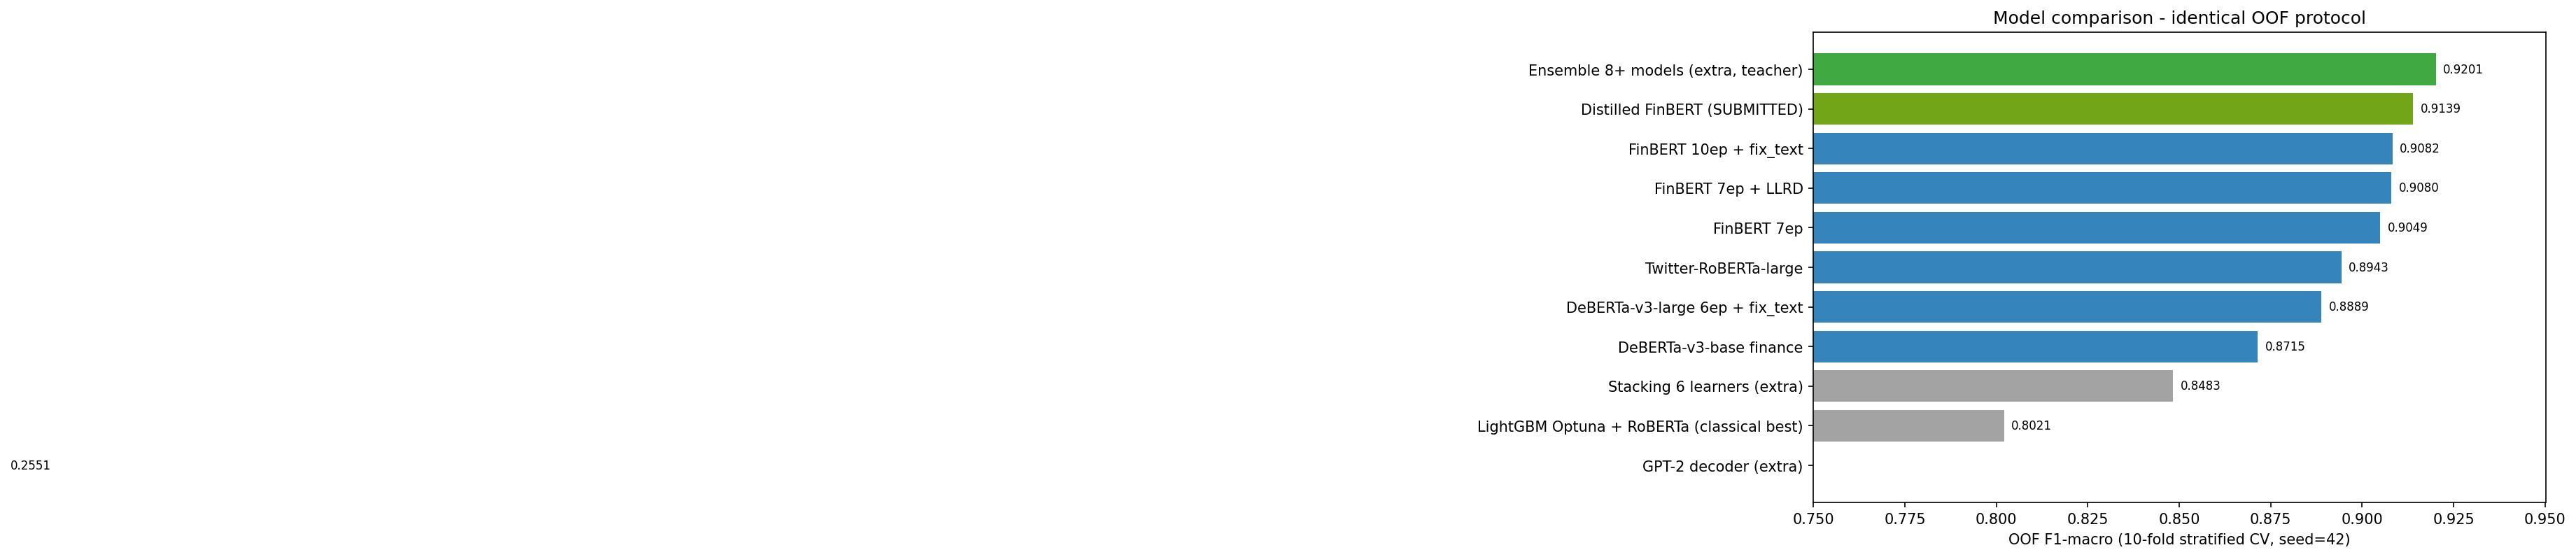
\includegraphics[width=0.84\linewidth]{report_results.png}
  \caption{Model comparison under the common OOF protocol (transformers: 10-fold; classical
  models: 5-fold). Green bars: the submitted ensemble and its distilled single-model variant.}
  \label{fig:results}
\end{figure}

\begin{table}[H]
  \centering
  \footnotesize
  \setlength{\tabcolsep}{5pt}
  \begin{tabularx}{\linewidth}{@{}>{\raggedright\arraybackslash}X r r r r r@{}}
    \toprule
    \tH{Model} & \tH{F1$_{\text{mac}}$} & \tH{$\sigma$} & \tH{Acc.} & \tH{Prec.} & \tH{Rec.} \\
    \gmid
    \rowcolor{lightgray} Ensemble, 8 encoders \textbar{} \textbf{submitted} & \textbf{0.9201} & --- & 0.9357 & 0.9097 & 0.9315 \\
    Distilled FinBERT student \emph{(extra)} & \distf & 0.0093 & \distacc & 0.9032 & 0.9258 \\
    FinBERT-fintwitter 10ep + fix\_text                 & 0.9082 & 0.0098 & 0.9293 & 0.9008 & 0.9163 \\
    FinBERT-fintwitter 7ep + LLRD                       & 0.9080 & 0.0099 & 0.9285 & 0.8967 & 0.9206 \\
    Twitter-RoBERTa-large topic-sent.\ (prev.\ subm.)   & 0.8943 & 0.0100 & 0.9141 & 0.8857 & 0.9036 \\
    DeBERTa-v3-large 6ep + fix\_text                    & 0.8889 & 0.0121 & 0.9107 & 0.8835 & 0.8945 \\
    Stacking-6 \textbar{} +fine-tuned \emph{(extra)}    & 0.8483 & 0.0073 & 0.8771 & 0.8271 & 0.8757 \\
    LightGBM Optuna + RoBERTa embeddings (best classical) & 0.8021 & --- & --- & --- & --- \\
    LightGBM + SBERT + SMOTE (Chawla et al., 2002)      & 0.7993 & --- & --- & --- & --- \\
    GPT-2 decoder fine-tuned \emph{(extra)}             & 0.7724 & 0.0159 & 0.8125 & 0.7475 & 0.8171 \\
    \bottomrule
  \end{tabularx}
  \caption{Top models by OOF macro-F1 (transformers: 10-fold; classical/stacking: 5-fold). The
  shaded row is the \textbf{submitted} ensemble; rows marked \emph{(extra)} are extra work.
  SMOTE improves the dense-embedding classical baseline by +0.6pp over class weighting but is
  irrelevant at transformer level, where the class-weighted loss already handles imbalance.}
  \label{tab:results}
\end{table}

\textbf{Key findings:} (1) dense transformer embeddings outperform sparse TF--IDF and static
embeddings across all model families; (2) end-to-end fine-tuning breaks the $\sim$0.80
frozen-embedding plateau; (3) within fine-tuning, \emph{domain match beats parameter count} ---
a 110M FinBERT beats a 435M DeBERTa-v3-large by $\sim$2pp; (4) text repair (fix\_text) is a free
+0.26pp; (5) ensemble knowledge survives compression into a single student model.

\subsection{Error Analysis}
Figure~\ref{fig:cm} shows the confusion matrix of the submitted ensemble. Per class it reaches F1 of
\textbf{0.895} (Bearish), \textbf{0.912} (Bullish) and \textbf{0.953} (Neutral). Errors concentrate
exactly where the EDA predicted (Section~2.4): the Neutral/directional boundary. Neutral tweets
drift into Bullish/Bearish when they report factual but direction-laden news (``price target
raised''), and directional tweets get softened into Neutral when the polarity is implicit. Bearish
remains the hardest class --- it is both the smallest (15.1\%) and the most mojibake-affected after
Neutral. On the held-out test set the model predicts 385 Bearish, 497 Bullish and 1{,}506 Neutral
(of 2{,}388) --- close to the training prior. Part of the residual error is the \emph{labels}, not
the model: the eight-encoder ensemble contradicts the gold label with $\geq$95\% confidence on
0.48\% of training tweets (e.g.\ ``Baird returns to Wingstop \emph{bull camp}'' is labelled
Neutral), a lower bound on annotation noise that no classifier can overcome. Three qualitative
failure modes remain: irony/sarcasm, mixed-signal tweets (`beats EPS but misses revenue'), and
truncated tweets whose decisive token was cut off --- the ceiling for text-only models on this
corpus.

\begin{figure}[H]
  \centering
  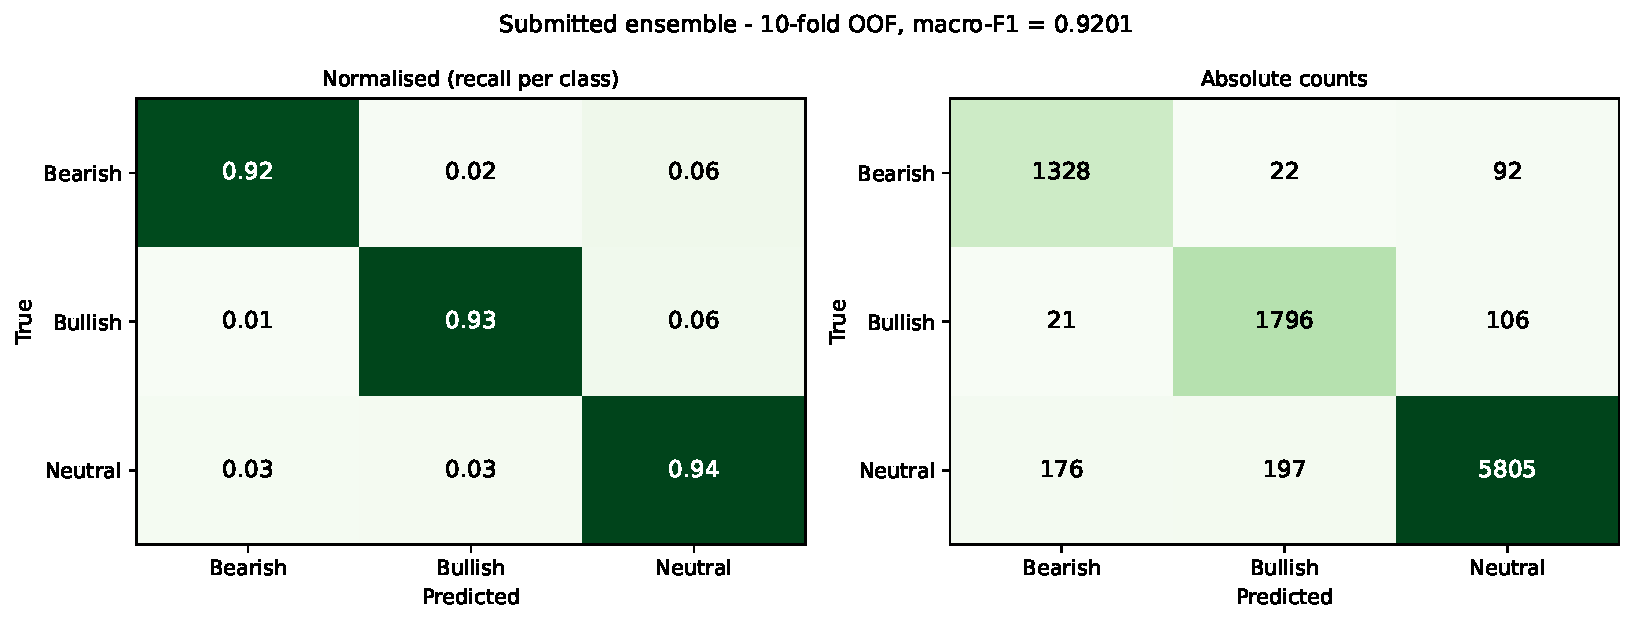
\includegraphics[width=0.96\linewidth]{confusion_matrix_ensemble.pdf}
  \caption{Confusion matrix of the submitted ensemble (normalised left, absolute counts
  right), from 10-fold out-of-fold predictions.}
  \label{fig:cm}
\end{figure}

\subsection{Statistical Significance and Calibration}
With only ten fold-level scores, fold-wise tests have low power: a Wilcoxon signed-rank test
between the two best individual encoders does not reach significance ($p=0.065$). We therefore
complement it with \emph{paired bootstrap} over the 9{,}543 OOF predictions (1{,}000 resamples),
which compares models on identical samples:
\begin{itemize}
  \item ensemble vs.\ best individual encoder: $\Delta$F1 95\% CI $=[+0.0066, +0.0172]$ --- significant;
  \item distilled student vs.\ best plain encoder: $[+0.0023, +0.0094]$ --- significant;
  \item best vs.\ second-best individual encoder: $[-0.0010, +0.0073]$ --- \emph{not} significant,
  confirming that single-encoder differences are within noise and the ensemble/distillation gains
  are the real levers.
\end{itemize}
Finally, a temperature-scaling search on the OOF probabilities finds $T{=}1.0$ optimal for every
fine-tuned model: training with label smoothing (0.05) already yields well-calibrated
probabilities (confidence-bucket accuracy matches predicted confidence within $\pm$3pp above 0.8),
so no post-hoc calibration is applied to the submission.

% ── 7. Agentic Workflow ──────────────────────────────────────────
\section{Extra Challenge 2 --- Agentic Workflow}
We implement a conversational agent that orchestrates three classifiers with \emph{non-trivial},
adaptive routing. The implementation lives in \nolinkurl{src/agent.py} and
\nolinkurl{notebooks/08_Agentic_Workflow.ipynb}. Following the course guideline on model choice,
the workflow uses \emph{open-source models exclusively} and requires no API key: the
conversational layer is a deterministic offline orchestrator, and the three tools are additionally
exposed as LangChain \texttt{Tool} objects as an integration point for locally-served open-source
LLMs in the ReAct style (Yao et al., 2022). The notebook includes both a scripted conversation
(reproducible under Restart \& Run All) and an optional live-chat cell where the grader can type
free-form phrases to the agent.

\subsection{Architecture and Routing}
The agent exposes three tools of escalating cost --- \tH{VADER} (lexical baseline,
$\sim$0.1\,ms), \tH{LightGBM+SBERT} (ML model trained in this project, $\sim$25\,ms) and
\tH{FinBERT-fintwitter} (the \emph{same domain backbone our submission fine-tunes}, used
zero-shot as the expert, $\sim$150\,ms) --- and routes adaptively.
SBERT is deliberately used for the middle-cost tool because it is fast and stable for
sentence-level semantic classification; the stronger but slower FinBERT expert is reserved for
disagreements. This is a cost-aware routing decision, not a claim that SBERT is the strongest
encoder overall.
The routing policy is:
\begin{itemize}
  \item VADER gives a quick lexical reading; if $|\text{compound}| > \tau$ it is trusted directly.
  The threshold $\tau$ is \emph{calibrated on data}, not hand-picked: a sweep on 400 held-out
  tweets finds the optimum at $\tau{=}0.85$ --- effectively discovering that the lexical tool
  should act as a cross-check rather than a decider, consistent with the VADER analysis of
  Section~2.4.
  \item Otherwise LightGBM+SBERT is consulted; if it agrees with VADER, that is the verdict.
  \item On \emph{disagreement}, the FinBERT expert is invoked as tie-breaker.
  \item Every verdict carries a reasoning trace with per-tool confidence and latency, and the
  session keeps conversational memory: free-form phrases are classified and \texttt{why} /
  \texttt{history} / \texttt{stats} / \texttt{compare:} follow-ups are supported.
\end{itemize}
Evaluation is \emph{leakage-aware}: the agent's LightGBM tool is retrained on 80\% of the corpus
and the agent is calibrated and evaluated only on the held-out 20\% (the public expert checkpoint
saw the train split, which we disclose; routing shares and latency are unaffected). On 400
held-out tweets the agent reaches accuracy 0.873 (macro-F1 0.833), resolving 44\% of tweets with
cheap tools and cutting mean latency by 18\% versus always calling the expert (0.915) --- the
quantified cost/accuracy trade-off that motivates agentic routing. The submitted ensemble
remains the accuracy reference; the agent demonstrates \emph{orchestration under a cost budget},
is deterministic, and is reproducible for the oral defence without any API key.

% ── 8. Conclusion ────────────────────────────────────────────────
\section{Conclusion}
This work delivers a complete NLP pipeline for financial tweet sentiment classification. Our
\textbf{submitted solution} --- a weighted soft-vote \textbf{ensemble} of eight fine-tuned
encoders --- achieves an out-of-fold macro-F1 of \textbf{0.9201} (accuracy 0.9357), a
\textbf{+0.118} gain over the 0.8021 classical baseline. Key contributions: (1) a text-quality audit
showing the corpus is corrupted at source, and a repair step (\texttt{ftfy} fix\_text) worth
+0.26pp at transformer level --- whereas \emph{destructive} preprocessing consistently hurts;
(2) systematic evaluation of 11 feature representations and 12 model families under a common
seeded protocol; (3) a nine-configuration transformer backbone search showing that
\emph{domain-matched pre-training beats parameter count} (110M FinBERT $>$ 435M DeBERTa-v3-large
by $\sim$2pp); (4, extra) knowledge distillation that compresses the submitted ensemble into a single
FinBERT (0.9139, retaining 44\% of the ensemble gain in one model); (5, extra) a
fine-tuned GPT-2 \emph{decoder} classifier (0.7724) with the finding that few-shot prompting of a
small decoder collapses to the majority class; (6, extra) an explainable, reproducible agentic
workflow. Future work could explore label-noise auditing of the Neutral boundary, domain-adaptive
pre-training on a larger financial-tweet corpus, and QLoRA fine-tuning of decoder LLMs.

% ── References ───────────────────────────────────────────────────
\section*{References}
{\small
Akiba, T., Sano, S., Yanase, T., Ohta, T., \& Koyama, M. (2019). Optuna: A next-generation
hyperparameter optimization framework. \emph{KDD 2019}.

Alammar, J., \& Grootendorst, M. (2024). \emph{Hands-On Large Language Models: Language
Understanding and Generation}. O'Reilly Media. [Course textbook.]

Antweiler, W., \& Frank, M. Z. (2004). Is all that talk just noise? The information content of
internet stock message boards. \emph{Journal of Finance}, 59(3), 1259--1294.

Araci, D. (2019). FinBERT: Financial sentiment analysis with pre-trained language models.
\emph{arXiv:1908.10063}.

Barbieri, F., Camacho-Collados, J., Espinosa Anke, L., \& Neves, L. (2020). TweetEval: Unified
benchmark and comparative evaluation for tweet classification. \emph{EMNLP-Findings 2020}.

Bollen, J., Mao, H., \& Zeng, X. J. (2011). Twitter mood predicts the stock market. \emph{Journal of
Computational Science}, 2(1), 1--8.

Brown, T. B., et al. (2020). Language models are few-shot learners. \emph{NeurIPS 2020}.

Chawla, N. V., Bowyer, K. W., Hall, L. O., \& Kegelmeyer, W. P. (2002). SMOTE: Synthetic minority
over-sampling technique. \emph{JAIR}, 16, 321--357.

Devlin, J., Chang, M.-W., Lee, K., \& Toutanova, K. (2019). BERT: Pre-training of deep
bidirectional transformers for language understanding. \emph{NAACL-HLT 2019}.

Go, A., Bhayani, R., \& Huang, L. (2009). Twitter sentiment classification using distant
supervision. \emph{Stanford CS224N Report}.

Hinton, G., Vinyals, O., \& Dean, J. (2015). Distilling the knowledge in a neural network.
\emph{arXiv:1503.02531}.

He, P., Gao, J., \& Chen, W. (2021). DeBERTaV3: Improving DeBERTa using ELECTRA-style pre-training
with gradient-disentangled embedding sharing. \emph{arXiv:2111.09543}.

Hutto, C. J., \& Gilbert, E. (2014). VADER: A parsimonious rule-based model for sentiment analysis
of social media text. \emph{ICWSM 2014}.

Loureiro, D., Barbieri, F., Neves, L., Espinosa Anke, L., \& Camacho-Collados, J. (2022). TimeLMs:
Diachronic language models from Twitter. \emph{ACL 2022 (System Demonstrations); arXiv:2202.03829}.

Manning, C. D., Raghavan, P., \& Sch\"utze, H. (2008). \emph{Introduction to Information Retrieval}.
Cambridge University Press.

Mikolov, T., Chen, K., Corrado, G., \& Dean, J. (2013). Efficient estimation of word representations
in vector space. \emph{arXiv:1301.3781}.

Pennington, J., Socher, R., \& Manning, C. D. (2014). GloVe: Global vectors for word representation.
\emph{EMNLP 2014}.

Radford, A., Wu, J., Child, R., Luan, D., Amodei, D., \& Sutskever, I. (2019). Language models are
unsupervised multitask learners. \emph{OpenAI Blog}.

Reimers, N., \& Gurevych, I. (2019). Sentence-BERT: Sentence embeddings using Siamese BERT-networks.
\emph{EMNLP 2019}.

Rennie, J. D., Shih, L., Teevan, J., \& Karger, D. (2003). Tackling the poor assumptions of Naive
Bayes text classifiers. \emph{ICML 2003}.

Sebastiani, F. (2002). Machine learning in automated text categorization. \emph{ACM Computing
Surveys}, 34(1), 1--47.

Speer, R. (2019). ftfy: Fixes text for you (Version 5.5). \emph{Zenodo}.
\texttt{doi:10.5281/zenodo.2591652}.

Wolpert, D. H. (1992). Stacked generalization. \emph{Neural Networks}, 5(2), 241--259.

Yao, S., Zhao, J., Yu, D., Du, N., Shafran, I., Narasimhan, K., \& Cao, Y. (2022). ReAct:
Synergizing reasoning and acting in language models. \emph{arXiv:2210.03629}.

Zhao, T. Z., Wallace, E., Feng, S., Klein, D., \& Singh, S. (2021). Calibrate before use: Improving
few-shot performance of language models. \emph{ICML 2021}.
}

\end{document}
